\documentclass{siproblemset}

\usepackage{multicol}
\usepackage{xcolor}

% SI Session Information
\course{MTH 1321}
\sessionnum{3}
\sessiondate{9/9/19}

\warmup{Concept Review}
\topic{What is a limit?}
\topic{Recognizing Continuity}
\topic{Determining Continuity}
\topic{Limits of Continuous Functions}
\topic{Indeterminate Forms}
\cooldown{Challenge Problems}

% Worksheet Information
\title{Continuity, Limits of Continuous\linebreak Functions, Indeterminate Forms}
\sections{Sections 2.4-2.5}
\withnamespace

\begin{document}
    \maketitle
    
    \activity{Warmup}{Concept Overview}{Work with a \textbf{partner} to answer these questions. Try not to use your notes.}{15 minutes}
    
    \frq{Define continuity in your own words and give the formal definition.}
    \tinyspace
    
    \frq{Give the formal definition of left- and right-continuity.}
    \nospace
    
    \frq{Name the three common types of discontinuities and sketch an example (graph) of each.}
    \smallspace
    
    \frq{Name some of the basic functions which are continuous on their domains.}
    \smallspace
    
    \frq{What are the indeterminate forms?}
    
    \pagebreak
    \activity{Activity 1}{Determining Continuity}{Find a \textbf{new partner with the same color worksheet as yours} to answer these questions. Try not to use your notes.}{30 minutes}
    
    \begin{multipartquestion}
        Determine the intervals of continuity on the following graphs. At points of discontinuity, state if the function is left- or right-continuous at that point and the type of discontinuity.
        \frq{}
        \mbox{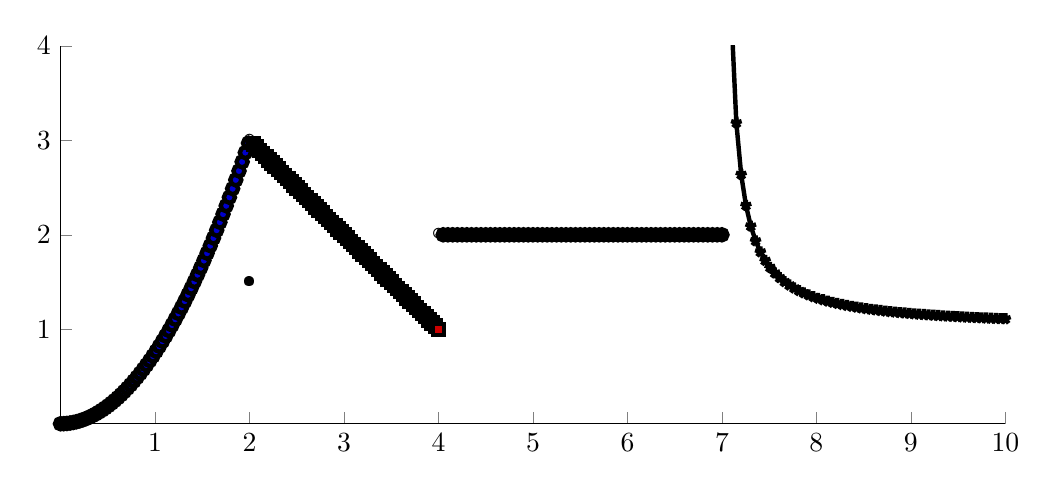
\begin{tikzpicture}[baseline=(current bounding box.north)]
            \begin{axis}[
                x=1.2cm,
                y=1.2cm,
                xmin=0,
                xmax=10,
                ymin=0,
                ymax=4,
                axis x line*=middle,
                axis y line*=middle,
                every axis plot/.append style={ultra thick},
                samples=60
                ]
                \addplot+[black, domain=0:1.99] {3/4*x^2};
                \node at (2,3) {$\circ$};
                \node at (2,1.5) {\textbullet};
                \addplot+[black, domain=2.04:4] {-x+5};
                \node at (4,1) {\textbullet};
                \node at (4,2) {$\circ$};
                \addplot+[black, domain=4.05:7] {2};
                \node at (7,2) {\textbullet};
                \addplot+[black, domain=7:10] {1/(3*(x-7))+1};
            \end{axis}
        \end{tikzpicture}}
        \tinyspace
        \frq{}
        \mbox{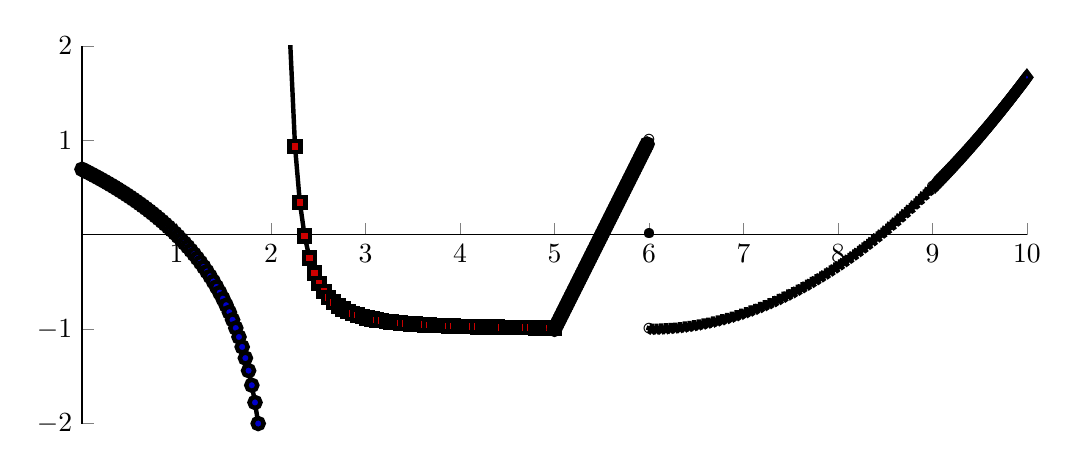
\begin{tikzpicture}[baseline=(current bounding box.north)]
            \begin{axis}[
            x=1.2cm,
            y=1.2cm,
            xmin=0,
            xmax=10,
            ymin=-2,
            ymax=2,
            axis x line*=middle,
            axis y line*=middle,
            every axis plot/.append style={ultra thick},
            samples=60
            ]
            \addplot+[black, domain=0:2] {ln(-(x-2))};
            \addplot+[black, domain=2:5,restrict y to domain =-5:5] {1/(8*(x-2)^2)-1};
            \node at (5,-1) {\textbullet};
            \addplot+[black, domain=5:5.98] {2*x-11};
            \node at (6,1) {$\circ$};
            \node at (6,0) {\textbullet};
            \node at (6,-1) {$\circ$};
            \addplot+[black, domain=6.03:8.97] {1/6*(x-6)^2-1};
            \node at (9,0.5) {$\circ$};
            \addplot+[black, domain=9.03:10] {1/6*(x-6)^2-1};
            \end{axis}
            \end{tikzpicture}}
        \tinyspace
    \end{multipartquestion}
\pagebreak
    \begin{multipartquestion}
        For your assigned problems, find the points of discontinuity of the given function. State the type of discontinuity and whether the function is left- or right-continuous at those point(s). If there are no points of discontinuity, state so explicitly. Justify your answers.
        \begin{multicols}{2}
            \frq{$h(x)=\dfrac{1}{2-|x|}$}
            \smallspace
            \frq{$f(x)=\tan(\sin x)$}
            \smallspace
            \frq{$s(t)=\lfloor t\rfloor~;~ 0\leq t\leq2$}
            \smallspace
            \frq{$g(x)=\dfrac{x+2}{3-x}$}
            \smallspace
            \frq{$b(z)=\ln|z+2|$}
            \smallspace
            \frq{$a(b)=3x^{2/3}-9x^3$}
            \smallspace
        \end{multicols}
        \smallspace
    \end{multipartquestion}
    
    \begin{multipartquestion}
        Find the values of $a$ and $b$ which make $f(x)$ continuous.
        \frq{$f(x)=\begin{cases}
            x^{-1} & x<-1\\
            ax+b & -1\leq x\leq \dfrac12\\
            x^{-1} & x > \dfrac12
            \end{cases}$}
        \frq{$f(x)=\begin{cases}
            a^x & x<-2\\
            -\dfrac1{2x} & -2\leq x< 3\\
            ab & x \geq 3
            \end{cases}$}
    \end{multipartquestion}

    \pagebreak
    \activity{Activity 2}{Limits of Continuous Functions and Indeterminate Forms}{Find a \textbf{group of three people all with the different color worksheets as yours} to answer these questions. Try not to use your notes.}{30 minutes}
    \begin{multipartquestion}
        Evaluate the following limits. If an indeterminate form is found, state the form and use algebra to solve the limit. If the limit does not exist, determine whether the one-sided limits exist (finite or infinite).
        \frq{$\lim\limits_{z\rightarrow8}\dfrac{z^3-64z}{z-8}$}
        \smallspace
        \frq{$\lim\limits_{x\rightarrow0}\dfrac{4^{2t}-1}{4^t-1}$}
        \smallspace
        \frq{$\lim\limits_{x\rightarrow36}\dfrac{\sqrt{x}-6}{x-36}$}
        \smallspace
        \frq{$\lim\limits_{t\rightarrow4}\dfrac{\sqrt{5-t}-1}{2-\sqrt{t}}$}
    \end{multipartquestion}
\pagebreak
    \begin{multipartquestion}
        Evaluate the following limits. If an indeterminate form is found, state the form and use algebra to solve the limit. If the limit does not exist, determine whether the one-sided limits exist (finite or infinite).
        \frq{$\lim\limits_{x\rightarrow0}\dfrac{\dfrac{1}{(h+2)^2}-\dfrac14}{h}$}
        \smallspace
        \frq{$\lim\limits_{k\rightarrow1}\left(\dfrac{1}{1-k}-\dfrac{2}{1-k^2}\right)$}
        \smallspace
        \frq{$\lim\limits_{\beta\rightarrow\frac{\pi}3}\dfrac{2\cos^2\beta+3\cos \beta-2}{2\cos \beta-1}$}
        \smallspace
        \frq{$\lim\limits_{\theta\rightarrow\frac\pi4}\dfrac{\sin x-\cos x}{\tan x - 1}$}
    \end{multipartquestion}
    \pagebreak
    \activity{Cooldown}{Challenge Problems}{Test your knowledge of these topics \textbf{alone} by attempting these challenge problems then sharing with the people around you.}{15 minutes}
    
    \begin{multipartquestion}
        Are the following functions continuous at $x=k$? If they are not, state the type of discontinuity and whether the function is left- or right-continuous (or neither) at $x=k$.
        \frq{$h(k)=5~;~\lim\limits_{x\rightarrow k^+}h(x)=5~;~\lim\limits_{x\rightarrow k^-}h(x)=2$}
        \tinyspace
        \frq{$f(k)=4~;~\lim\limits_{x\rightarrow k}f(x)=4$}
        \tinyspace
        \frq{$g(k)=6~;~\lim\limits_{x\rightarrow k}g(x)=-2$}
        \tinyspace
        \frq{$q(k)=3~;~\lim\limits_{x\rightarrow k^+}h(x)=-6~;~\lim\limits_{x\rightarrow k^-}h(x)=-\infty$}
        \tinyspace
    \end{multipartquestion}

    \begin{multipartquestion}
        Find all values of $c$ such that the following limits exist.
        \frq{$\lim\limits_{x\rightarrow c}\dfrac{x^2-5x-6}{x-c}$}
        \tinyspace
        \frq{$\lim\limits_{x\rightarrow c}\left(\dfrac{1}{x-1}-\dfrac{c}{x^3-1}\right)$}
    \end{multipartquestion}
\end{document}